% icai2017.sty uses the next packages:
% geometry, [utf8]inputenc, [T1]fontenc, [english]babel, graphicx, [intlimits]amsmath, amssymb, amsthm, caption, titlesec, url
%
% Defined theorem-like environments:
% definition, theorem, lemma, remark, example, corollary, proof
%
% You can define new theorem-like environment in the following way (see amsthm.sty):
% \newtheorem{prob}[theorem]{Problem}

\documentclass{article}
\usepackage{icai2017}
\usepackage{graphicx}

\usepackage{array}
\newcolumntype{L}[1]{>{\raggedright\let\newline\\\arraybackslash\hspace{0pt}}m{#1}}
\newcolumntype{C}[1]{>{\centering\let\newline\\\arraybackslash\hspace{0pt}}m{#1}}
\newcolumntype{R}[1]{>{\raggedleft\let\newline\\\arraybackslash\hspace{0pt}}m{#1}}

\newtheorem{prob}[theorem]{Problem}

\title{Cross Translational Unit Analysis in Clang Static Analyzer: Prototype and measurements}
\author{D\'aniel Krupp\inst1,\ Zolt\'an Porkol\'ab\inst1,\ Gy\"orgy Orb\'an\inst1\\
        G\'abor Horv\'ath\inst2,\ Zolt\'an Gera\inst2}
\institute{\inst1Ericsson Ltd., \inst2E\"{o}tv\"{o}s Lor\'{a}nd University, Faculty of Informatics\\
             \inst1\url{daniel.krupp@ericsson.com}, 
             \inst1\url{zoltan.porkolab@ericsson.com},
             \inst1\url{gyorgy.orban@ericsson.com},
             \inst2\url{xazax@caesar.elte.hu}, 
             \inst2\url{gerazo@caesar.elte.hu}}
             
\begin{document}
\maketitle

% %%%%%%%%%%%%%%%%%%%%%%%%%%%%%%%%%%%%%%%%%%%%%%

\begin{abstract}
Today Clang SA can perform (context-sensitive) inter-procedural analysis for 
C,C++ and Objective C files by ''inlining'' 
the called function into the callers' context. This means that that the full 
calling context
(assumptions about the values of function parameters, global variables) is passed when 
analyzing the called function and
then the assumptions about the returned value is passed back to the caller. 
This works well for function calls within a
translation unit (TU), but when the symbolic execution reaches a function that 
is implemented in another TU, the analyzer engine 
skips the analysis of the called function definition. In particular,
assumptions about references and pointers passed as function 
parameters get invalidated, and the return value of the function will be unknown.
Losing information this way may lead to false positive
and false negative findings.

The cross translation unit (CTU) feature allows the analysis of called 
functions even if the definition of the function is external to the currently 
analyzed TU. This would allow detection of bugs in library functions stemming
from incorrect usage (e.g. a library assumes that the user will free a memory 
block allocated by the library), and allows for more precise analysis
of the caller in general if a TU external function is invoked
(by not losing assumptions).

We implemented (based on the prototype by A. Sidorin, et al.~\cite{artemctu})
the Cross Translation Unit analysis feature for Clang SA (4.0) and evaluated 
its performance on various open source projects. In our presentation, we show 
that by using the CTU feature we found many new true positive reports and 
eliminated some false positives in real open source projects. We show that 
while the total analysis time increases to 2-3 times, the execution remains
scalable in the number of CPUs. We also point out how the analysis
coverage changes that may lead to the loss of reports compared to the 
non-CTU baseline version.
\keywords C++ programming language, static analysis, cross translation unit analysis
\end{abstract}

% %%%%%%%%%%%%%%%%%%%%%%%%%%%%%%

\section{Description of the CTU prototype}
Our method being worked on enables CTU analysis 
by inlining external function definitions using clang's existing ASTImporter 
(see \cite{astimporter}) functionality.
One of our goals was to have minimal, isolated, and lightweight changes.
We added less than 300 lines of code to the clang codebase 
(1200 lines of code including the support utilities that are 
  separate executables and tests). 

\subsection{Two-pass analysis}
To perform the analysis, we need to run clang on the whole source code two times 
(see Figure~\ref{figctu}).
%[Cross Translation Analysis Overview]

\subsubsection*{1st pass}
The first analysis phase generates 3 important outputs: AST dump of all
translation units, a map file for functions with external linkage, the global call graph.
The AST binary (using the {\tt clang -emit-ast}) 
of each TU is generated into a temporary directory. 
The mangled name and location of all externally linkable functions 
are collected into the function definition index (externalFnMap.txt). 

The global call graph of the program is stored in another text file.

\begin{figure}[h!]
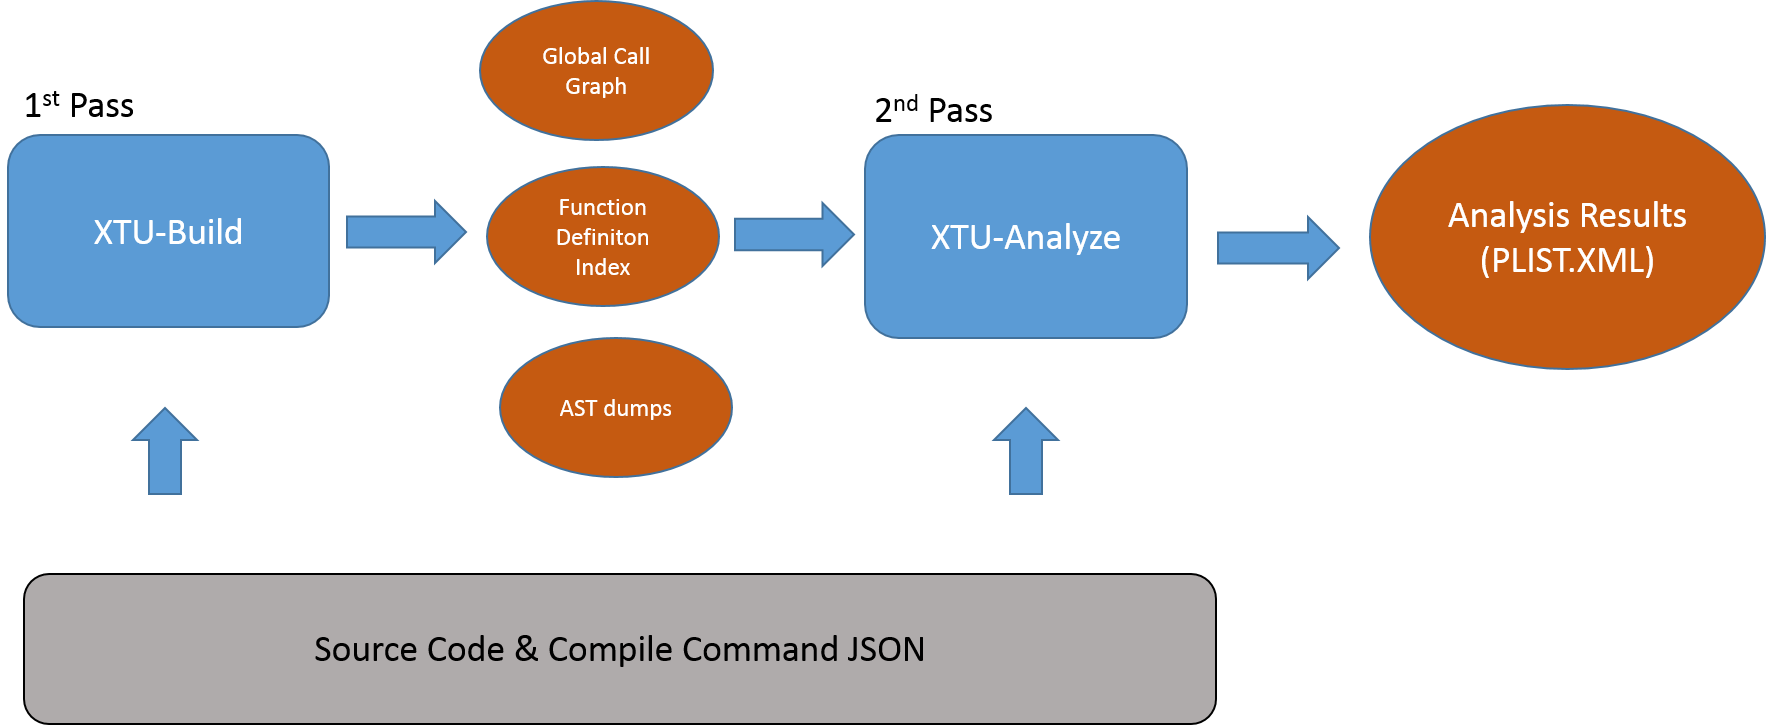
\includegraphics[width=\textwidth]{images/ctu.png}
\caption{2-Pass CTU analysis overview}
\label{figctu}
\end{figure}

\subsubsection*{2nd pass}
The Clang Static Analyzer is run for all translation units. When a TU external
function is reached during the analysis, the location of the definition 
of that function is looked up in the function definition index and the 
definition is imported from the containing AST binary into the caller's context
using the \texttt{ASTImporter} library.

\subsection{Traversal of the call graph}
In the non-CTU analysis, functions that are not called from within the TU are
analyzed first as ``top-level'' functions and all functions that are
non-top-level are only analyzed in a call context (as they are called). 
In our CTU implementation, when analyzing a source file, we start the analysis
from the same top-level functions as the original non-CTU method even if a given
function is called from another TU (according to the global call graph). 
The practical reason for choosing this strategy is that if the project 
contains test cases then library functions would only be analyzed with 
the concrete test values which would result in loss of generality of the analysis. 

The source code of the prototype is available in this clang GitHub
fork~\cite{ctugithub}.


\section{Results on Open Source projects}
We have analyzed many open source projects 
(FFmpeg, tmux, curl, Vim, PostgreSQL, \dots) using CTU and
found many new true positive reports (see Table~\ref{tblfindings}.

The measurements were taken using clang-4.0 as the baseline and the same
clang-4.0 with the CTU patch. Only the (stable) checkers enabled by default
were switched on. To compare and view the results we have used CodeChecker~\cite{codechecker}.


\begin {table}[h!]
\centering
\begin{tabular}{| L{1.6cm}| C{1.6cm} | C{1.6cm} | C{1.6cm} | C{1.6cm} | C{1.6cm} |}
  \hline
  Analyzed project& All non-CTU Findings (baseline)&All CTU Findings&New CTU findings & Disappeared findings & Successfully / Failed to analyze
  \\
  \hline
  \hline
  FFmpeg& 339& 399 & 101& 41& 1555/8 files \\
  \hline
  tmux& 49& 77 & 29& 1 & 133/0 files \\
  \hline
  curl& 7& 11& 4& 0 & 280/13 files\\
  \hline  
\end{tabular}
\caption{CTU and non-CTU results comparison}
\label{tblfindings}
\end{table}


\subsection{Quality of new results}
The new analysis method has found significant number of new results on all projects. 
The number of findings increased by $17\%$ to $50\%$.
We examined the new findings in detail and most of them are true positive.
According to our evaluation of the CTU analysis, the quality of the introduced results
weren't worse than the non-CTU results (there was no precision loss at CTU boundary).

The CTU analysis has revealed many new bugs that require lengthy symbolic analysis,
such as memory leak problems (\texttt{unix.Malloc}), dereference of null pointers
(\texttt{core.NullDereference}, \texttt{core.NonNullParamChecker},
\texttt{core.CallAndMessage}) \\ and usage of uninitialized values
(\texttt{core.uninitialized.Assign}, \\ \texttt{core.uninitialized.Branch},
\texttt{core.UndefinedBinaryOperatorResult}).

See for example distribution of new findings for FFmpeg project in 
Table~\ref{tblffmpegbugs}.

\begin {table}[h!]
\centering
\begin{tabular}{| l|| c |}
\hline
Checker ID&                          Number of new findings \\
\hline
\hline
core.CallAndMessage                &  5 \\
\hline
core.DivideZero                    & 5 \\     
\hline
core.NonNullParamChecker           & 12 \\     
\hline
core.NullDereference               & 18 \\     
\hline
core.UndefinedBinaryOperatorResult & 21 \\     
\hline
core.uninitialized.Assign          & 11 \\     
\hline
core.uninitialized.Branch          & 6  \\     
\hline
unix.Malloc                        & 23 \\
\hline
\end{tabular}
\caption{Distribution of new bug reports on the FFmpeg project}
\label{tblffmpegbugs}
\end{table}

We expected that the bug path length of the new results would be longer 
than the results in the baseline, due to the long traversal of function 
calls into external source files (see Table~\ref{tblbpl}). This assumption turned out to be true as
the median of the bug path length of new bugs is 16 compared to the non-CTU
case of 7 (for FFmpeg). However in practice 16 long bug paths are still 
manageable for programmers.

\begin {table}[h!]
\centering
\begin{tabular}{| C{2cm}|| C{2cm} | C{2cm} |C{2cm} |C{2cm} |}
  \hline
  Analyzed project & Median of bug path length (BPL) in baseline&Median of BPL CTU&Median of BPL of new findings&Median of BPL of disappeared findings\\
  \hline
  \hline
  FFmpeg&7&9&16&14\\
  \hline
  tmux&16&16&17&6\\
  \hline
  curl& 1&1&12&n.a.\\
  \hline  
\end{tabular}
\caption{CTU and non-CTU Bug Path Length comparison}
\label{tblbpl}
\end{table}

Some of the results disappeared compared to the baseline analysis. 
We are still investigating the reason for this, but we primarily 
suspect two reasons:

\begin{enumerate}
  \item The analysis coverage of the base file somewhat changed,
        because in some cases the analysis node budget is consumed
        by the traversal of longer CTU paths instead of paths inside the base
        file. It must be noted that in the non-CTU case the paths inside the
        base file have inherently imprecise assumptions about external
        functions.

  \item It is also possible that some of the findings disappeared
        compared the baseline because they were false positives as they were
        based on false assumptions about unknown external functions. However
        we think this is only case to a less extent as Clang SA checkers are written
        conservatively to report less false positives.
\end{enumerate}

Detailed analysis of the results can be found in the following
pages:~\cite{ffmpegres},~\cite{tmuxres},~\cite{curlres}.

\subsection{Performance}
In general the analysis time (including both analysis passes) 
increased $\sim 2$ to $\sim 2.5$ times of the baseline non-CTU analysis time on all analyzed
projects (see Table~\ref{tbltime}). The increment is due to the first analysis phase and the extra effort
of loading the definitions of external functions from disk during the
analysis. The measurements were performed on the same machine having 16 CPU cores.
The resource requirements of the new analysis is not dramatic and the solution is
similarly scalable to multiple CPUs as the baseline, because all build actions
are analyzed independently.

\begin {table}[h!]
\centering
\begin{tabular}{| L{2cm}| C{2cm} | C{2cm} | C{2cm}|}
  \hline
  Analyzed project& Analysis Time (baseline) {\scriptsize [s]} &Analysis Time CTU (1st + 2nd Phase) {\scriptsize [s]}\\
  \hline
  \hline
  FFmpeg& 318&44+693\\
  \hline
  tmux& 39&4+75\\
  \hline
  Curl& 32&6.5+54\\
  \hline  
\end{tabular}
\caption{CTU and non-CTU analysis time comparison}
\label{tbltime}
\end{table}

\section{Future work}

\begin{itemize}
  \item The current CTU prototype is only usable for C projects.
    We have experienced many crashes and assertion failures of the
    \texttt{ASTImporter} for C++ projects.
    \texttt{ASTImporter} needs to be improved to handle C++ language elements
    and constructs better.

  \item \emph{Do we lose true positives and coverage in the base file?}
    We plan to measure coverage and experiment with different strategies
    to build the exploded graph. One simple strategy might be to bound
    the number of file traversals.

  \item Some path sensitive based bug reports have the so-called uniquing locations that help
    to differentiate them. These currently work for single TUs only.
    We would like to extend them to multiple TUs.

  \item During the analysis, we need to store the dumped ASTs temporarily.
    We plan to decrease the disk usage by compressing AST dumps or
    storing them more efficiently.
\end{itemize}

\section{Credits}
This work is based on earlier work of Aleksei Sidorin,\ Artem Dergachev,\ 
et al.\@ See \url{http://lists.llvm.org/pipermail/cfe-dev/2015-October/045730.html}

\begin{thebibliography}{9}
\bibitem{ccelte} Cross-TU Analysis results on open source projects, \url{http://cc.elte.hu/}

\bibitem{artemctu} Artem Dergachev, Aleksei Sidorin: \emph{Cross TU Analysis for Clang 3.4}
  \url{http://lists.llvm.org/pipermail/cfe-dev/2015-October/045730.html}

\bibitem{ericssonctu} Ericsson CTU open source repository, \url{https://github.com/dkrupp/clang/tree/ctu-master}
\bibitem{ctugithub} \url{https://github.com/dkrupp/clang/tree/ctu-master}
\bibitem{ffmpeg} FFmpeg project, \url{https://github.com/FFmpeg/FFmpeg}
\bibitem{tmux} tmux project, \url{https://github.com/tmux/tmux}
\bibitem{curl} curl project, \url{https://github.com/curl/curl}
\bibitem{astimporter} \texttt{ASTImporter}, \url{http://clang.llvm.org/doxygen/classclang_1_1ASTImporter.html}
\bibitem{ffmpegres} FFmpeg CTU Results, {\small \url{https://github.com/dkrupp/clang/wiki/FFMpeg-XTU-Analysis}}
\bibitem{tmuxres} tmux CTU Results, \url{https://github.com/dkrupp/clang/wiki/TMUX-XTU-Analysis}
\bibitem{curlres} curl CTU Results, \url{https://github.com/dkrupp/clang/wiki/Curl-XTU-Analysis}
\bibitem{codechecker} CodeChecker, \url{https://github.com/Ericsson/codechecker}
\end{thebibliography}
\end{document} 
